\chapter{Building an electronic thermometer}
We built an electronic thermometer. This was done by using the PT100, a platinum resistor with a well known thermal coefficient $\alpha$. We made a fixed current pass through the PT100 and registered the voltage of each rsistor end, then we amplified this signal and with an intrumentation amplifier we imposed the final output to be 0 V when the temperature was 0 \degree C. The objective was to have a voltage that could've been easily converted to a temperature by multipling it to a coefficient $\eta = 10 \frac{\degree C}{\text{V}}$


\section{Materials}
\begin{itemize}
\item Operational amplifiers OP07
\item Instrumentation amplifier (INA) AD622
\item Precision +5V Voltage Reference REF02
\item Thermoresistor PT100
\item Resistors, trimmers
\item Power supply RIGOL DP831A
\item Waveform generator RIGOL DG1032
\item Multimeter RIGOL DM3068
\item Transistor 2N2222
\end{itemize}
The resistors used were all with an uncertainty of 5\%
\section{Electronic thermometer}
Firstly we measured the resistance of the PT100 with two methods. With the standard two wires measure, by adding on each end two 10 $\Omega$ resistor to simulate the presence of parassite resisor. We measured $R_t = 13x \Omega$ which converted with $T = \frac{R_t - R_0}{R_0 \alpha}$\footnote{ $R_0$ is the PT100's resistance at 0 $\degree C$ and $\alpha$ is the thermal coefficient, that is around $0.003850 \degree C^{-1}$  }
gave us $80 xx \degree C$. We then used the 4 wires configuration and meausured $R_t = 10x \Omega$ and the temperaure of  $\degree C$.
\begin{figure}[H]
\centering
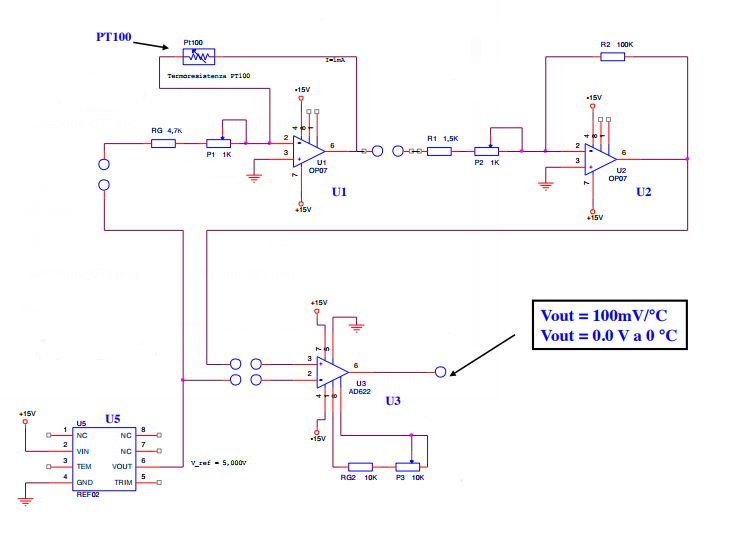
\includegraphics[width=.7\textwidth]{6/circuit.png}
\end{figure}
For build the thermometer circuit first we turned the resistor's mesurament in a voltage's mesurament, we've done this simply using a fixed current in the PT100.
For letting flow a fixed current in the PT100 we needed a highly stable current generator. The one we built needed a stable input voltage, for this  reason we used the REF02 that had an output of $4.9993 \pm 0.0003$ V. Then we measured the current passing through the the PT100 and we made it as close as 1mA by tweaking the trimmer attached to the inverting pin.\\
For having the output with the format required in the abstract we needed the total gain of the circuit to be $G_{tot} = \frac{100 \frac{mV}{\degree C}}{\alpha} = 259.740$. Because we also needed to set the output to 0 mV at 0 \degree C we decided to first amplify the voltage on the ends of the PT100 by a factor of 50 and then use this output in the differential amplifier, that had a gain of 5.195, this allowed us to take the first amplified signal and compare it with the signal that would had been at $0\degree C$ (in our case exactly 5V).\\
For the amplifier stage we used a OP07 in inverting configuration. For setting the gain of the amplifier stage we used an input voltage of around 100 mV and we made the output signal as close as possible to 5 V, by using a trimmer.\\
In the last stage of the circuit we used AD622 that had to be tested and needed some getting used to, for this reason we built a bridge circuit with attached the AD622. We used two resistors of 100k$\Omega$, one of $1k\Omega$ and one of $100 \Omega$ with in series a trimmer, we used also a resistance of 51.1 $\Omega$ (1\% of uncertainty) to set the gain of the AD622 to 1000 (989.3 to be exact). By changing the resistance of the trimmer we were able to null the output voltage.
\begin{figure}[H]
\centering
\begin{circuitikz}
%ponte
\draw(0,0);
\draw(0,6.7)--(0,7.2);
\node[above] at (0,7.2) {$v_{+}$};
\draw(-1,6.7)--(1,6.7);
\draw(-1,6.7)--(-1,6.2);
\draw(1,6.7)--(1,6.2);
\draw (-1,6.2) to[R,l^=$R_1$](-1,4.7);
\draw (1,6.2) to[R,l^=$R_2$](1,4.7);
\draw(-1,4.7)--(-1,3.5);
\draw(1,4.7)--(1,3.5);
\draw (-1,3.5) to[R,l^=$R_4$](-1 ,2);
\draw (1,3.5) to[vR,l^=$R_3$](1,2);
\draw(-1,2)--(-1,1.5);
\draw(1,2)--(1,1.5);
\draw(-1,1.5)--(1,1.5);
\node[sground] at (0,1.5) {};
%opamp
\draw(-1,4.69)--(4,4.69);
\draw(1,3.71)--(4,3.71);
\node[op amp] (opamp) at (5,4.2) {};
\draw(5,5.3)--(5,4.7);
\node[above] at (5,5.3) {$+v_{cc}$};
\draw(5,3.0)--(5,3.7);
\node[below] at (5,3.0) {$-v_{cc}$};
\node[right] at (6.19,4.2) {$v_{out}$};
%gain resistance
\draw(4.3,5.1)--(4.3,6.3);
\draw (4.3,6.3) to[R,l^=$R_G$](5.5,6.3);
\draw(5.5,6.3)--(5.5,4.4);

\end{circuitikz}
\caption{Testing bridge}\label{Ponte}
\end{figure}


After this test we felt confident to build a differational amplifier with a gain of 5.195, by putting to ground the inverting signal and using a sine wave signal of 100mV on the non-inverting pin and changing the output by tweaking the trimmer attached to the $R_G$ pin.\\
At last we connected all the circuits together. The signal from the current generator was used as input signal in the amplifier and the output of the amplifier was placed on the non-inverting pin of the differential amplifier and on the inverting pin was placed the voltage generated from the REF02. we connected the output to the multimeter and changed the setting to output 1 \degree C to for each 100mV in the output. The value visible was about 25 \degree C and we made sure that  it was changing by heating the PT100.

\section{The P of PID}
\begin{figure}[H]
\centering
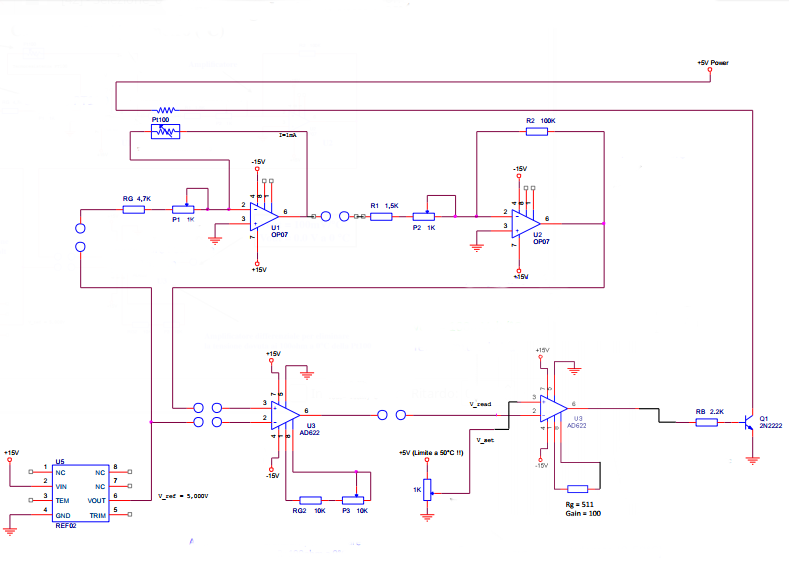
\includegraphics[width=.8\textwidth]{6/circuit2.png}
\end{figure}
We connected the output of the thermometer to a differential amplifier with $G=100$. So we compered the temperature with a reference chosen by us, by connecting the non inverting pin to a trimmer. The output of the INA was connected to the base of a NPN transistor using a resistor in between. The transitor controlled a power circuit made with a small resistence $R$ with a voltage of 5V taken from the agilent generator. The PT100 was placed attached to the small resistor, so we measured the temperature of $R$. When the temperature set by the trimmer is different frome the one measured with the PT100, the difference is amplified and converted to a current in the power circuit which heat up the resistor until the the difference in temperature is nullified. The current flowing in $R$ is proportional to the temperature difference. The differential amplifier had a saturation voltage of around 10, so the amplification of 100 allowed us to control the temperature on a range of 1 \degree C (100 mV).\\
For the current's measure we used a tester ICE placed between $R$ and the transistor. During the test, when we changed the desired temperature using the trimmer, we saw the current raise and then make damped oscillations towards a stable current.
